\documentclass{article}
\usepackage{neurips_2026}
\usepackage[utf8]{inputenc}
\usepackage[T1]{fontenc}
\usepackage{hyperref}
\usepackage{url}
\usepackage{booktabs}
\usepackage{amsfonts,amsmath,amssymb,amsthm}
\usepackage{nicefrac}
\usepackage{microtype}
\usepackage{xcolor}
\usepackage{graphicx}
\usepackage{enumitem}
\setlist{nosep,leftmargin=*}

\newtheorem{proposition}{Proposition}
\newtheorem{remark}{Remark}
\newcommand{\Delta}{\Delta}
\renewcommand{\Delta}{\Delta}
\newcommand{\simplex}{\Delta^{K-1}}
\newcommand{\hh}{\hat h}
\newcommand{\XC}{\mathrm{XC}}
\newcommand{\Gini}{G}
\newcommand{\PP}{\mathbb{P}}
\newcommand{\EE}{\mathbb{E}}

\title{How Should We Evaluate Conformal Prediction for Compositional Outputs? Geometry, Reference Measures, and Conditional Coverage}

\author{Anonymous Authors}

\begin{document}
\maketitle

\begin{abstract}
Many predictors output a composition, a non-negative vector summing to one (softmax probabilities, topic or label proportions), and the target itself may be a composition (e.g.\ a human label distribution). Split conformal prediction gives distribution-free \emph{marginal} coverage for any set-valued summary of such outputs, but the choice of nonconformity score changes the \emph{shape} of the region on the simplex, and there is no agreed way to compare the resulting regions. We study how to evaluate conformal methods on the simplex. We (i) show that marginal coverage is blind to the geometry of the score and that comparing efficiency requires an explicit reference measure: we prove that the Aitchison measure has density $1/(\sqrt K\prod_i p_i)$ w.r.t.\ Lebesgue measure, so any Euclidean-type region touching the boundary has \emph{infinite} Aitchison volume, while Aitchison balls have vanishing Lebesgue volume near the boundary; (ii) show analytically and numerically that single-test-set binomial intervals for coverage are anti-conservative, with a closed-form false-alarm rate $2\{1-\Phi(1.96/\sqrt{1+T/(n+2)})\}$ ($T$ test points, $n$ calibration points), and recommend calibration-resampling confidence intervals; (iii) derive why unnormalised $L_2$-type scores under Dirichlet/multinomial noise undercover high-Gini predictions ($\EE\|y-\mu\|^2=\Gini(\mu)/(\phi+1)$) and check this against simulation. In a benchmark of 12 scores on 6 synthetic generators (300 calibration draws each) and on CIFAR-10H human label distributions, all scores attain the nominal marginal coverage, but their efficiency rankings differ across generators and, within a generator, across reference measures (in 14--37 of 66 score pairs, depending on the generator, two statistically significant orderings are reversed by changing the measure); conditional coverage over the simplex differs by up to 10 percentage points. No score dominates; the best choice depends on the noise model and on the measure the user cares about. We give conditions under which these conclusions should not be extrapolated.
\end{abstract}

\section{Introduction}
A predictor whose output is a composition $\hh\in\simplex=\{p\in\mathbb R^K_{\ge0}:\sum_ip_i=1\}$ --- a softmax vector, a vector of topic proportions, an estimated mixture --- is rarely used without some statement of uncertainty. When the \emph{target} $Y\in\simplex$ is itself compositional (a distribution of human annotator labels, a mixture of components in a sample), a natural uncertainty statement is a region $C(x)\subset\simplex$ that contains $Y$ with probability $1-\alpha$. Conformal prediction \citep{vovk2005algorithmic,lei2018distribution,angelopoulos2021gentle} delivers such regions with finite-sample, distribution-free \emph{marginal} guarantees under exchangeability. It does so for \emph{any} nonconformity score, and the literature offers many: Euclidean residuals, divergences, log-ratio distances \citep{aitchison1982statistical}, likelihood-based scores, normalised or Mondrian variants. The guarantee therefore cannot be used to choose between them, and the community has no shared protocol for doing so on the simplex, where the geometry is non-Euclidean, boundaries and exact zeros are common, and noise is heteroscedastic by construction (a composition near a vertex has little room to vary).

\textbf{Research question.} \emph{How should the reliability of conformal prediction regions for compositional outputs be evaluated, and under which conditions is one method preferable to another?} We break this down into five hypotheses that guided the experimental design (all stated before the main runs; each can be refuted):
\begin{itemize}
\item[\textbf{H1}] Realised coverage of split conformal regions follows its exact Beta law for every score, so deviations from nominal in an experiment are explained by calibration-set randomness and not by the score.
\item[\textbf{H2}] Evaluation by coverage alone is uninformative about geometry; efficiency comparisons depend on the measure used to size regions, and rankings can reverse.
\item[\textbf{H3}] Scores whose geometry matches the noise model (KL/Hellinger for Dirichlet or count noise; Aitchison/Mahalanobis for logistic-normal noise) are the most efficient under the data distribution.
\item[\textbf{H4}] Unnormalised Euclidean-type scores violate conditional coverage along the Gini/concentration axis in a way predictable from the noise model; normalisation or Mondrian calibration reduces this at a price in variance (small $n$) or efficiency.
\item[\textbf{H5}] Reporting a binomial confidence interval for coverage on one calibration split is anti-conservative; the unit of replication must be the calibration draw.
\end{itemize}
\textbf{Contributions.} (1) An evaluation protocol for simplex-valued conformal regions combining calibration-resampled coverage intervals, a data-driven cross-coverage efficiency measure and a family of Dirichlet reference-measure volumes, and conditional-coverage diagnostics along simplex-specific axes (\S\ref{sec:method}). (2) Four propositions with proofs (\S\ref{sec:theory}), each checked numerically: Beta law and invariance; Aitchison--Lebesgue density and its consequences for volume comparisons; Gini scaling of Dirichlet residuals; and the false-alarm rate of the naive single-split protocol. (3) A benchmark of 12 scores on 6 generators plus CIFAR-10H (\S\ref{sec:exp}) with calibration-resampling confidence intervals, paired tests and Holm correction. (4) A statement of when the conclusions do and do not extend (\S\ref{sec:disc}).

\section{Related work}
\textbf{Conformal prediction.} Split (inductive) conformal prediction \citep{papadopoulos2002inductive,lei2018distribution} gives marginal coverage with an exact Beta distribution of the realised coverage over calibration sets \citep{vovk2012conditional}; \citet{angelopoulos2021gentle} give a tutorial. Full conformal and jackknife+ \citep{barber2021predictive} trade computation for sample efficiency; we use split conformal throughout and do not study these. Locally weighted scores \citep{lei2018distribution}, conformalised quantile regression \citep{romano2019conformalized}, and Mondrian/class-conditional calibration \citep{vovk2005algorithmic,ding2023class} target conditional coverage, which cannot be achieved exactly in a distribution-free way \citep{barber2021limits}; multivalid methods \citep{jung2023batch} offer group-conditional guarantees. Weighted conformal prediction handles covariate shift when the density ratio is known \citep{tibshirani2019conformal}. \textbf{Classification and distribution-valued outputs.} For classifiers, conformal sets over \emph{labels} use scores such as $1-\hh_y$ \citep{sadinle2019least}, cumulative mass \citep{romano2020classification}, and regularised variants \citep{angelopoulos2021uncertainty}; \citet{stutz2022learning} optimise efficiency end-to-end and \citet{cresswell2024conformal} study downstream effects of set-valued outputs. \citet{javanmardi2024conformalized} predict credal sets of distributions. Our setting differs: the object being covered is a point on the simplex (a distribution), not a label. KL$(y\|\hh)$ with one-hot $y$ equals $-\log\hh_y$, so our score family contains the standard least-ambiguous-set score as a special case. \textbf{Compositional data.} The Aitchison geometry \citep{aitchison1982statistical} and isometric log-ratio coordinates \citep{egozcue2003isometric} give the simplex a vector-space structure; we use them both as a family of scores and as a measure on the simplex, and show their interaction with the usual Euclidean geometry matters for \emph{evaluation}. We are not aware of a systematic comparison of conformal methods for simplex-valued outputs; we do not claim novelty for individual conformal methods, but for the evaluation analysis.

\section{Setting, methods and evaluation protocol}\label{sec:method}
\textbf{Setting.} Data $(X_i,Y_i)\in\mathcal X\times\simplex$ are exchangeable. A predictor $\hat f$ trained on a training split gives $\hh(x)=\hat f(x)\in\simplex$. A second \emph{auxiliary} split is used only to fit score hyper-parameters (covariance, scale model, Dirichlet precision), so that the score is fixed before calibration. For a score $s(\hh,y,x)$ and calibration scores $S_1..S_n$, $\hat q$ is the $\lceil(n+1)(1-\alpha)\rceil$-th smallest ($+\infty$ if it exceeds $n$) and $C(x)=\{u\in\simplex:s(\hh(x),u,x)\le\hat q\}$. Mondrian variants calibrate $\hat q_g$ per group $g(\hh(x))$.

\textbf{Scores} (Table~\ref{tab:scores}). Euclidean-type: $L_2,L_1,L_\infty$; Hellinger; $\mathrm{KL}(y\|\hh)$; Aitchison distance $\|\mathrm{clr}(y_\delta)-\mathrm{clr}(\hh_\delta)\|_2$ with additive zero replacement $p\mapsto(p+\delta)/(1+K\delta)$, $\delta=10^{-3}$ unless stated; Mahalanobis distance in clr space with the aux-split residual covariance; negative Dirichlet log-density with fitted precision (an HPD-type score; zeros replaced as above); $L_2/\sqrt{\Gini(\hh)}$ with $\Gini(p)=1-\sum_ip_i^2$ (motivated in Prop.~\ref{prop:gini}); $L_2$ locally weighted by a ridge-regression estimate of $\log$-residual \citep{lei2018distribution}; $L_2$ with Mondrian calibration by $\arg\max\hh$ or by Gini quartile of $\hh$.
\begin{table}[t]\centering\small
\caption{Scores. $\hh$ predicted composition, $y$ target. All are fixed functions of $(\hh,y,x)$ given the training/aux splits.}\label{tab:scores}
\begin{tabular}{ll|ll}\toprule
$L_2,L_1,L_\infty$ & $\|y-\hh\|_{2,1,\infty}$ & Mahal-clr & $\sqrt{r^\top\Sigma^+r},\ r=\mathrm{clr}(y_\delta)-\mathrm{clr}(\hh_\delta)$\\
Hellinger & $\|\sqrt y-\sqrt{\hh}\|_2$ & DirNLL & $-\log\mathrm{Dir}(y_\delta;\hat\phi\,\hh_\delta)$\\
KL & $\sum_iy_i\log(y_i/\hh_i)$ & $L_2/\sqrt{\Gini}$ & $\|y-\hh\|_2/\sqrt{\Gini(\hh)}$\\
Aitchison & $\|\mathrm{clr}(y_\delta)-\mathrm{clr}(\hh_\delta)\|_2$ & $L_2/\hat\sigma$; Mondrian & learned scale; per-group $\hat q_g$\\\bottomrule
\end{tabular}\end{table}

\textbf{Evaluation protocol.} Given a calibration draw $\mathcal D_c$ (and hence $C$), we measure on a large test set:
\begin{itemize}
\item \textbf{Coverage and its uncertainty.} Realised coverage $\mathrm{Cov}(\mathcal D_c)=\PP(Y\in C(X)\mid\mathcal D_c)$. We replicate over \emph{independent calibration draws} ($R=300$ per configuration; 1000 for the coverage-law study) and report means with 95\% CIs over draws. Methods are compared on identical draws (paired tests, Wilcoxon, Holm correction).
\item \textbf{Efficiency, two families.} (a) \emph{Cross-coverage} $\XC=\PP(Y'\in C(X))$ with $Y'$ an independent draw from the marginal of $Y$ (we pair $x_i$ with $y_j$, $j\neq i$, of the test set). It measures how often a region contains an unrelated plausible target and uses the data distribution as its reference. (b) \emph{Dirichlet reference volume} $V_a=\EE_X\,\PP_{U\sim\mathrm{Dir}(a\mathbf 1)}(U\in C(X))$; $a=1$ is the normalised Lebesgue measure on the simplex and $a\to0$ approaches the Aitchison measure (Prop.~\ref{prop:measure}). We report $a\in\{0.1,0.3,1,3\}$.
\item \textbf{Conditional coverage.} Coverage within quintiles of $\Gini(\hh(X))$ (the natural axis of heteroscedasticity on the simplex), summarised by the worst-bin gap $\max_b|\mathrm{Cov}_b-(1-\alpha)|$ (noise floor in our setting: $0.024$, simulated for an ideal method with $n=500$ and 800 test points per bin), and by the minimum bin coverage. We also record coverage by $\arg\max\hh$ class.
\end{itemize}

\section{Theory}\label{sec:theory}
All proofs are in Appendix~\ref{app:proofs}; numerical checks in \S\ref{sec:exp} and Appendix~\ref{app:theory}.
\begin{proposition}[Coverage law and invariance]\label{prop:beta}
If calibration and test scores are exchangeable with no ties, $\mathrm{Cov}(\mathcal D_c)\sim\mathrm{Beta}(n+1-l,l)$, $l=\lfloor(n+1)\alpha\rfloor$, with mean $\lceil(n+1)(1-\alpha)\rceil/(n+1)$ and variance $\approx\alpha(1-\alpha)/(n+2)$ \citep{vovk2012conditional}. For any bijection $\psi$ of $\simplex$ (e.g.\ clr/ilr), the region built from the score $s\circ\psi^{-1}$ on $\psi(Y)$ is $\psi(C)$, and $Y\in C\iff\psi(Y)\in\psi(C)$: coverage is identical in every parametrisation; only the family of regions (and hence efficiency) depends on the geometry. In particular the Aitchison score is the Euclidean score in ilr coordinates.
\end{proposition}
\begin{proposition}[Measures on the simplex]\label{prop:measure}
Let $A$ be Lebesgue measure in ilr coordinates (the Aitchison measure) and $\lambda$ Lebesgue measure in coordinates $p_{1:K-1}$. Then $dA(p)=\big(\sqrt K\prod_{i=1}^Kp_i\big)^{-1}d\lambda(p)$. Consequently (a) if a region $R$ contains a relatively open neighbourhood of a point of a facet $\{p_i=0\}$ (with the other coordinates positive), $A(R)=\infty$; this holds for the $L_p$, Hellinger and KL regions as soon as $\hat q>\hh_i(x)$ (resp.\ the analogous threshold) for some $i$; (b) an Aitchison ball of radius $\rho$ around $\hh$ has $\lambda(B)\le\sqrt K e^{2K\rho}\prod_i\hh_i\cdot\omega_{K-1}\rho^{K-1}$, which tends to $0$ as $\min_i\hh_i\to0$ for fixed $\rho$. With $\mathrm{Dir}(a\mathbf 1)$ reference measures, $d\mathrm{Dir}_a/dA\propto\prod_ip_i^{a}$, so $a=1$ is Lebesgue and $a\downarrow0$ approaches (improper) $A$.
\end{proposition}
\begin{proposition}[Gini scaling]\label{prop:gini}
If $y\sim\mathrm{Dir}(\phi\mu)$ then $\EE\|y-\mu\|_2^2=\Gini(\mu)/(\phi+1)$; if $y=\mathrm{Mult}(N,\mu)/N$ then $\EE\|y-\mu\|_2^2=\Gini(\mu)/N$. As $\phi\to\infty$, $\sqrt{\phi+1}(y-\mu)\Rightarrow\mathcal N(0,\mathrm{diag}(\mu)-\mu\mu^\top)$, whose trace is $\Gini(\mu)$. Hence, with a pooled threshold $\hat q$, the conditional coverage of the $L_2$ score at $x$ is approximately $\PP(\sum_j\lambda_j(\mu)Z_j^2\le(\phi+1)\hat q^2)$, $Z_j$ i.i.d.\ $\mathcal N(0,1)$, $\lambda_j$ the eigenvalues of $\mathrm{diag}(\mu)-\mu\mu^\top$ ($\sum_j\lambda_j=\Gini(\mu)$): it is decreasing in the first-order scale $\Gini(\mu)/(\phi+1)$, so $L_2$ over-covers low-Gini and under-covers high-Gini predictions. Dividing by $\sqrt{\Gini(\hh)}$ removes the first-order dependence for constant $\phi$.
\end{proposition}
\begin{proposition}[Naive single-split evaluation]\label{prop:naive}
Suppose the realised coverage is approximately $\mathcal N(e,\sigma_n^2)$, $\sigma_n^2=\alpha(1-\alpha)/(n+2)$, $e$ its mean, and one evaluates it on $T$ i.i.d.\ test points with the Wald interval $\hat c\pm1.96\sqrt{\hat c(1-\hat c)/T}$. Then the probability that the interval excludes $e$ is, to first order,
$\;2\{1-\Phi(1.96/\sqrt{1+T/(n+2)})\}$, which tends to $1$ as $T\to\infty$ at fixed $n$. Intervals over $R$ independent calibration draws have the nominal level.
\end{proposition}

\section{Experiments}\label{sec:exp}
\textbf{Synthetic generators} ($K=5$, covariates $x\in\mathbb R^5$ standard normal, $n_{tr}=1000$, aux $500$, calibration pool $2000$, test $4000$; fixed population structure, fresh data per replicate). Mean $\mu(x)=\mathrm{softmax}(A^\top x+b)$. \emph{dir\_homo}: $\mathrm{Dir}(20\mu)$. \emph{dir\_het}: precision $20e^{1.2x_0}$. \emph{dir\_sparse}: $\mathrm{Dir}(3\mu)$ (many near-zero components). \emph{dir\_nl}: Dirichlet with a nonlinear mean the linear predictor cannot fit (bias). \emph{lnorm\_het}: logistic-normal $\mathrm{softmax}(\eta+\sigma(x)L\varepsilon)$, $\sigma(x)=0.5e^{0.5x_0}$. \emph{mult50}: $\mathrm{Mult}(50,\mu)/50$ (about 28\% exact zeros). The predictor is softmax regression fitted by cross-entropy to the soft targets. \textbf{Real data.} CIFAR-10H \citep{peterson2019human}: for each of the 10{,}000 CIFAR-10 test images \citep{krizhevsky2009learning}, the empirical distribution of $\approx$50 human labels ($80.6\%$ of entries are exactly zero); the predictor is a CIFAR-10 classifier trained on the 50{,}000 training images (details in \S\ref{sec:cifar}). Each replicate re-draws aux/calibration/test from a random permutation of the 10{,}000 images. Unless stated: $\alpha=0.1$, $n=500$, $R=300$, seeds are functions of (experiment, generator, replicate) so every table is regenerated exactly by the supplied scripts.

\textbf{H1: realised coverage follows the Beta law for every score.} For 60 (generator, $n\in\{50,200,1000\}$, score) cells without Mondrian calibration ($R=1000$ draws, 20{,}000 test points each), the Kolmogorov--Smirnov test against $\mathrm{Beta}(n+1-l,l)$ rejects at 5\% in 2 of 60 cells (3.3\%, none at 1\%), no cell has $|z|>3$ for the mean, the largest deviation of mean coverage from its Beta mean is 0.0025, and the SD ratio to theory is in $[0.947,1.053]$ (Fig.~\ref{fig:law}a). Mondrian variants over-cover as expected from rounding in smaller groups (mean coverage 0.911/0.909 vs.\ 0.9005 at $n=200$, dir\_het) and at $n=30$ Mondrian-by-Gini covers 0.966 (many groups have $\hat q=\infty$, i.e.\ the region is the whole simplex). \textbf{H1 supported.}

\textbf{H5: the naive protocol is anti-conservative.} Fig.~\ref{fig:law}b simulates one test set of size $T$ per calibration draw and asks whether the 95\% Wald interval excludes the exact expected coverage. With $n=200$ and $T=2000$ it does in 55.7\% of cases (Prop.~\ref{prop:naive} predicts 55.3\%); with $T=10^4$ and $n=50$, in 89.2\% (88.8\%); the prediction is within 0.03 everywhere except $n=50,T=500$ (57.9\% vs 54.7\%, where the Beta law is visibly non-normal). Intervals over $R\in\{10,30\}$ calibration draws exclude it in 4.5--6.6\% of cases. A difference of 0.5 percentage points in coverage between two scores on one split is therefore not evidence of anything at $n\le10^3$. \textbf{H5 supported.}

\begin{figure}[t]
\centering
\begin{minipage}[t]{0.62\linewidth}\centering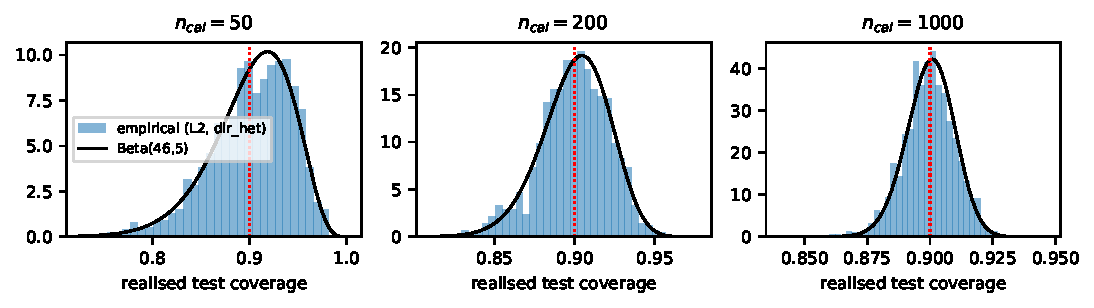
\includegraphics[width=\linewidth]{../figs/fig_covlaw.pdf}\\{\small (a) realised coverage vs.\ Beta law}\end{minipage}\hfill
\begin{minipage}[t]{0.36\linewidth}\centering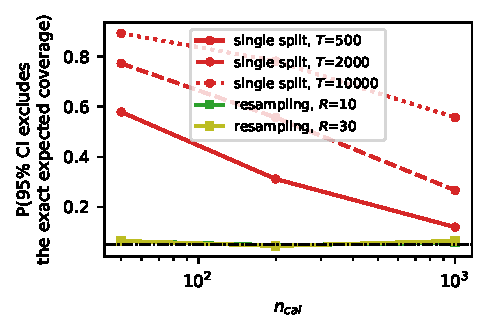
\includegraphics[width=\linewidth]{../figs/fig_protocol.pdf}\\{\small (b) single split vs.\ resampling}\end{minipage}
\caption{(a) Histograms of realised coverage (1000 calibration draws, $L_2$, dir\_het) and the exact Beta law. (b) Probability that a 95\% CI excludes the exact expected coverage, averaged over scores $\{L_2,\mathrm{KL},\mathrm{Aitchison}\}$ and generators $\{$dir\_het, mult50$\}$; dash-dot line: 5\%.}\label{fig:law}
\end{figure}

\begin{figure}[t]\centering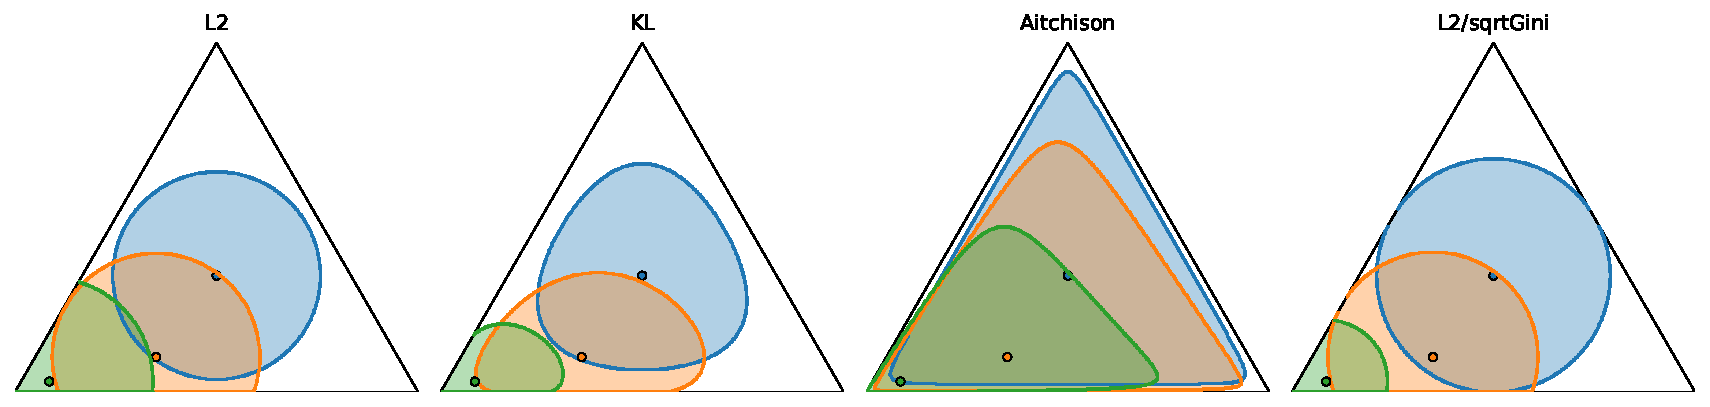
\includegraphics[width=\linewidth]{../figs/fig_ternary.pdf}
\caption{Regions on the simplex ($K=3$, dir\_het-type generator, $n=2000$, $\alpha=0.1$) at three predicted compositions (dots). Thresholds $\hat q$: $L_2$ 0.36, KL 0.21, Aitchison 2.51, $L_2/\sqrt{\Gini}$ 0.50. All regions have the same marginal coverage.}\label{fig:tern}\end{figure}

\textbf{All scores reach the nominal marginal level, so coverage cannot rank them.} Mean realised coverage at $n=500,\alpha=0.1$ is within $[0.899,0.902]$ for every non-Mondrian score and generator (95\% CIs $\le0.0018$), and within $[0.9500,0.9551]$ at $\alpha=0.05$ and $[0.8005,0.8044]$ at $\alpha=0.2$ for all scores (the upper ends correspond to Mondrian rounding). The regions themselves differ greatly (Fig.~\ref{fig:tern}).

\textbf{H2/H3: efficiency depends on the generator and on the measure used.} Table~\ref{tab:eff} shows XC and the uniform-reference volume $V_1$. By XC, the best score is Hellinger (dir\_homo), DirNLL (dir\_het), Aitchison (dir\_sparse), KL (dir\_nl, mult50) and Mahalanobis-clr (lnorm\_het); for logistic-normal noise the clr-space scores are 5--10$\times$ more efficient than $L_2$ in XC (0.014 vs.\ 0.150), as H3 predicts, whereas for Dirichlet and multinomial noise KL/Hellinger win and the clr-space scores are about 2--7$\times$ \emph{worse} than KL on mult50 (XC 0.098 vs.\ 0.013) --- an Aitchison score cannot resolve exact zeros, where the choice of $\delta$ matters (below). Under the uniform measure ($V_1$) the picture reverses for log-ratio scores: Aitchison/Mahalanobis have $V_1\approx0.14$--$0.21$ on Dirichlet/multinomial generators against $0.01$--$0.07$ for most others, consistent with Prop.~\ref{prop:measure}(b)'s reverse statement that Aitchison-type regions are large in Lebesgue terms in the interior while vanishing near the boundary; conversely DirNLL, an HPD region which is Lebesgue-volume-optimal when the density is correct, is best at $V_1$ in 5/6 generators (all but lnorm\_het). Fig.~\ref{fig:rank} gives ranks under five measures. Within each generator, among the 66 score pairs, the number for which one measure significantly (Holm, $p<0.05$, paired Wilcoxon) prefers $A$ and another prefers $B$ is 35 (dir\_homo), 37 (dir\_het), 24 (dir\_sparse), 26 (dir\_nl), 14 (lnorm\_het), 26 (mult50). \textbf{H2 supported; H3 supported for the matched pairs described, with the DirNLL/HPD exception noted.} A caveat: XC is not measure-free; it uses the marginal of $Y$, which makes it a statement about \emph{this} data distribution.

\begin{table}[t]\centering\scriptsize\setlength{\tabcolsep}{3pt}
\caption{Efficiency at $n=500$, $\alpha=0.1$ (mean of 300 draws; max 95\% CI half-width 0.0034 (XC), 0.0038 ($V_1$); bold = best; full CIs in Appendix). Top: cross-coverage XC. Bottom: volume fraction $V_1$ under the uniform measure on the simplex. Lower is better.}\label{tab:eff}
\begin{tabular}{lrrrrrr}
\toprule
score & dir\_homo & dir\_het & dir\_sparse & dir\_nl & lnorm\_het & mult50 \\
\midrule
L2 & $0.068$ & $0.095$ & $0.236$ & $0.202$ & $0.150$ & $0.033$ \\
L1 & $0.065$ & $0.088$ & $0.225$ & $0.182$ & $0.135$ & $0.032$ \\
Linf & $0.072$ & $0.101$ & $0.248$ & $0.218$ & $0.160$ & $0.035$ \\
Hellinger & $\mathbf{0.031}$ & $0.057$ & $0.162$ & $0.122$ & $0.081$ & $0.016$ \\
KL & $0.034$ & $0.055$ & $0.175$ & $\mathbf{0.120}$ & $0.078$ & $\mathbf{0.013}$ \\
Aitchison & $0.064$ & $0.098$ & $\mathbf{0.144}$ & $0.144$ & $0.029$ & $0.098$ \\
Mahal-clr & $0.064$ & $0.099$ & $0.147$ & $0.143$ & $\mathbf{0.014}$ & $0.097$ \\
DirNLL & $0.041$ & $\mathbf{0.055}$ & $0.170$ & $0.132$ & $0.080$ & $0.024$ \\
L2/$\sqrt{\mathrm{Gini}}$ & $0.055$ & $0.090$ & $0.236$ & $0.206$ & $0.140$ & $0.022$ \\
L2/learned-sigma & $0.069$ & $0.092$ & $0.323$ & $0.242$ & $0.167$ & $0.025$ \\
L2-Mondrian(argmax) & $0.071$ & $0.099$ & $0.246$ & $0.208$ & $0.168$ & $0.035$ \\
L2-Mondrian(gini) & $0.059$ & $0.100$ & $0.243$ & $0.208$ & $0.159$ & $0.024$ \\
\bottomrule
\end{tabular}\\[3pt]
\begin{tabular}{lrrrrrr}
\toprule
score & dir\_homo & dir\_het & dir\_sparse & dir\_nl & lnorm\_het & mult50 \\
\midrule
L2 & $0.027$ & $0.051$ & $0.300$ & $0.256$ & $0.120$ & $0.007$ \\
L1 & $0.021$ & $0.038$ & $0.238$ & $0.196$ & $0.087$ & $0.005$ \\
Linf & $0.035$ & $0.065$ & $0.337$ & $0.296$ & $0.149$ & $0.009$ \\
Hellinger & $0.016$ & $0.037$ & $0.220$ & $0.163$ & $0.052$ & $0.007$ \\
KL & $0.013$ & $0.025$ & $0.143$ & $0.110$ & $0.038$ & $0.004$ \\
Aitchison & $0.137$ & $0.206$ & $0.464$ & $0.401$ & $0.037$ & $0.205$ \\
Mahal-clr & $0.139$ & $0.206$ & $0.463$ & $0.397$ & $\mathbf{0.017}$ & $0.205$ \\
DirNLL & $\mathbf{0.005}$ & $\mathbf{0.006}$ & $\mathbf{0.013}$ & $\mathbf{0.034}$ & $0.027$ & $\mathbf{0.002}$ \\
L2/$\sqrt{\mathrm{Gini}}$ & $0.035$ & $0.071$ & $0.306$ & $0.273$ & $0.130$ & $0.009$ \\
L2/learned-sigma & $0.065$ & $0.090$ & $0.388$ & $0.332$ & $0.189$ & $0.015$ \\
L2-Mondrian(argmax) & $0.032$ & $0.060$ & $0.318$ & $0.274$ & $0.137$ & $0.009$ \\
L2-Mondrian(gini) & $0.036$ & $0.080$ & $0.330$ & $0.281$ & $0.177$ & $0.009$ \\
\bottomrule
\end{tabular}
\end{table}

\begin{figure}[t]\centering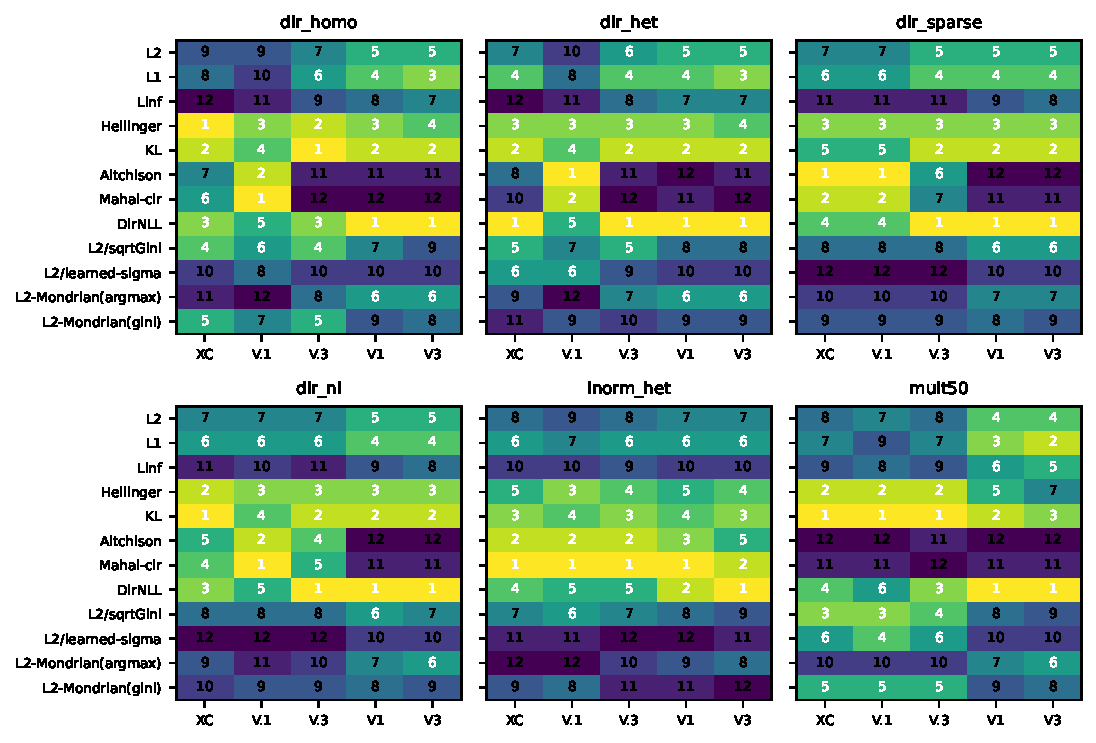
\includegraphics[width=0.78\linewidth]{../figs/fig_ranks.pdf}
\caption{Rank of each score (1 = smallest region) under XC and Dirichlet reference volumes $V_{0.1},V_{0.3},V_1,V_3$, per generator. Columns disagree within generators.}\label{fig:rank}\end{figure}

\textbf{H4: conditional coverage along the Gini axis.} Fig.~\ref{fig:cond} shows coverage by $\Gini(\hh)$ quintile. $L_2$ over-covers low-Gini predictions (0.98--1.00 in the first quintile) and under-covers the highest (0.81 on dir\_homo and mult50), matching Prop.~\ref{prop:gini}: at $\phi=20$ the Gaussian approximation predicts bin coverages $(0.998,0.964,0.904,0.862,0.822)$ against $(0.988,0.949,0.894,0.836,0.834)$ simulated (Appendix~\ref{app:theory}), and $\EE\|y-\mu\|^2$ matches $\Gini(\mu)/(\phi+1)$ within 5\% at $\phi\in\{3,10,20,100\}$ (4000 points). $L_2/\sqrt{\Gini}$ reduces the worst-bin gap from 0.101 to 0.032 (dir\_homo) and from 0.108 to 0.031 (mult50); Aitchison/Mahalanobis, KL and Mondrian-by-Gini are also better than $L_2$ in most generators (Appendix Table). The gap of the best methods ($0.03$--$0.05$) is still above the 0.024 noise floor: these scores equalise the first-order scale but not the shape. The ridge-learned scale $\hat\sigma$ \emph{over}-corrects (coverage 0.97 at the highest quintile) and is no better than $L_2$ by the gap on four generators. $L_2$-Mondrian by $\arg\max$ does not help along the Gini axis (gap 0.083--0.103 for $L_2$ and 0.083--0.103 Mondrian-by-argmax in dir\_het/mult50) as expected, since the groups are not aligned with the heteroscedasticity. With few calibration points Mondrian-by-Gini is worse than a plain score (Fig.~\ref{fig:ncal}, Appendix): its gap is 0.107 at $n=30$ and overtakes $L_2/\sqrt{\Gini}$ only for $n\gtrsim500$. \textbf{H4 supported; the learned normaliser is not reliably better than the closed-form one here.}
\begin{figure}[t]\centering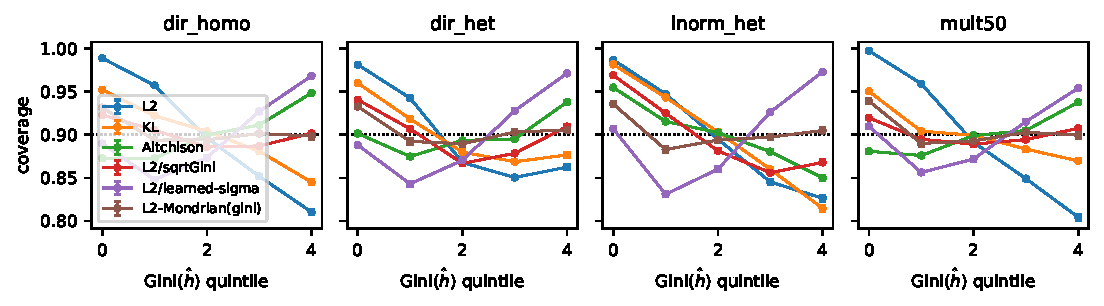
\includegraphics[width=\linewidth]{../figs/fig_cond.pdf}
\caption{Coverage by $\Gini(\hh)$ quintile (error bars: 95\% CI over 300 draws; dotted: nominal).}\label{fig:cond}\end{figure}

\textbf{Robustness 1: covariate shift.} We shift the test distribution of $x_0$ (which drives the noise precision in dir\_het). Unweighted split conformal loses coverage when the test distribution moves towards the noisy region (shift $-1$: $L_2$ 0.759, KL 0.757, Aitchison 0.750, $L_2/\sqrt{\Gini}$ 0.754; shift $-1.5$: 0.65--0.69) and over-covers towards the quiet region (shift $+1$: 0.975). The learned-scale score is much more robust (0.876 and 0.864), because its coverage is closer to conditional on the shifted covariate. Weighted conformal \citep{tibshirani2019conformal} with the exact density ratio restores 0.898--0.907 for all five scores (Fig.~\ref{fig:shift}). The conclusion about robustness depends on the shifted variable being one the normaliser has access to (here $x_0$ enters its features); for CIFAR-style data where only $\hh$ is available, it need not hold.
\begin{figure}[t]\centering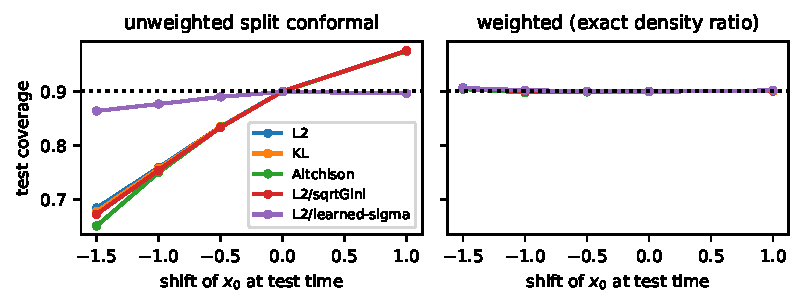
\includegraphics[width=0.62\linewidth]{../figs/fig_shift.pdf}
\caption{Coverage under covariate shift of $x_0$ (dir\_het, $n=1000$, 300 draws; CIs smaller than markers).}\label{fig:shift}\end{figure}

\textbf{Robustness 2: exact zeros and the Aitchison $\delta$.} On mult$N$ with $N\in\{5,\dots,1000\}$ (Appendix Fig.~\ref{fig:multN}) coverage remains nominal (0.899--0.902) for all scores and $\delta$, but the Aitchison efficiency depends strongly on $\delta$: at $N=50$, XC is 0.225, 0.097, 0.023, 0.019 for $\delta=10^{-4},10^{-3},10^{-2},10^{-1}$ (KL: 0.013), and at $N=1000$ 0.025, 0.0011, 0.0003, 0.0009 (KL 0.0002). Marginal coverage gives no warning that the score is mis-tuned. Choosing $\delta$ must be part of the evaluation, and ideally uses the aux split.

\subsection{Real data: CIFAR-10H}\label{sec:cifar}
\input{cifar_section.tex}

\section{Discussion and limitations}\label{sec:disc}
\textbf{What we can and cannot conclude.} (i) Marginal coverage of split conformal regions on the simplex is valid for all scores tested and its randomness is exactly the Beta law; evaluation papers should report intervals over calibration draws. (ii) Efficiency rankings are a property of (score, noise model, reference measure). No score was uniformly best, and the common practice of reporting a single volume or set-size number hides rank reversals that are frequent (14--37 of 66 pairs). (iii) Conditional coverage along Gini is explained by the noise scale; closed-form normalisation is a cheap, effective first-order fix. We advise reporting at least two reference measures including a data-driven one.

\textbf{Limitations.} Synthetic conclusions hold for the six generators with $K=5$, $d=5$, a well-behaved softmax-regression predictor, and $n_{tr}=1000$; we did not vary $K$ (only a $K=3$ illustration), the predictor class, or the training-set size, and results for $K\gg10$ are unverified. Efficiency measures depend on Monte-Carlo reference samples (600 test points $\times$ 200 uniform draws per measure) and conditional-coverage gaps are subject to a 0.024 noise floor; the group-conditional evidence concerns the Gini and $\arg\max$ axes only, not all subgroups, and conditional validity is not guaranteed by any method here. The theory is first-order: Prop.~\ref{prop:gini} is an asymptotic approximation (checked at $\phi\ge3$), Prop.~\ref{prop:naive} uses a normal approximation to the Beta law (error up to 0.03 for $n=50$). Calibration and test data are exchangeable except in the shift experiment, which uses exact density ratios; estimated weights, label shift, and temporal shift are untested. Real-data evidence comes from a single dataset (CIFAR-10H) with a weak, non-deep predictor (see \S\ref{sec:cifar}) and may not extend to modern deep classifiers. We did not study full conformal, jackknife+, or multivalid methods, or set-valued \emph{label} predictions, and we did not tune any score beyond $\delta$ and ridge strength. Finally, we did not evaluate downstream effects on human decisions \citep{cresswell2024conformal}. These conclusions should not be extrapolated to non-exchangeable data, much larger $K$, or predictors whose outputs are saturated (near one-hot), where ties and zero replacement dominate.

\bibliographystyle{plainnat}
\bibliography{refs}

\appendix
\section{Proofs}\label{app:proofs}
\paragraph{Proof of Proposition~\ref{prop:beta}.} Let $F$ be the (continuous) c.d.f.\ of the score and $U_i=F(S_i)$, i.i.d.\ uniform for i.i.d.\ data. With $k=\lceil(n+1)(1-\alpha)\rceil\le n$, $\hat q=S_{(k)}$ and $\mathrm{Cov}(\mathcal D_c)=\PP(S_{n+1}\le S_{(k)}\mid\mathcal D_c)=F(S_{(k)})=U_{(k)}\sim\mathrm{Beta}(k,n+1-k)$, and $n+1-k=\lfloor(n+1)\alpha\rfloor=l$. The mean is $k/(n+1)$ and the variance $k\,l/((n+1)^2(n+2))\approx\alpha(1-\alpha)/(n+2)$. For a bijection $\psi$ with $s'(\psi(h),\psi(y))=s(h,y)$, $s'(\psi(h),\psi(Y_i))=S_i$, so thresholds coincide and $\{u:s'(\psi(h),u)\le\hat q\}=\psi(\{u:s(h,u)\le\hat q\})$; $Y\in C\iff\psi(Y)\in\psi(C)$. The Aitchison score is $\|\mathrm{ilr}(y_\delta)-\mathrm{ilr}(\hh_\delta)\|_2$ since ilr is an isometry of clr.\hfill$\square$

\paragraph{Proof of Proposition~\ref{prop:measure}.} Let $V\in\mathbb R^{(K-1)\times K}$ have orthonormal rows spanning $\mathbf 1^\perp$, so $\mathrm{ilr}(p)=V\log p$. In the free coordinates $\tilde p=p_{1:K-1}$, $p=E\tilde p+e_K$ with $E=[I_{K-1};-\mathbf 1^\top]$, hence $\partial\log p/\partial\tilde p=P^{-1}E$ with $P=\mathrm{diag}(p)$ and the Jacobian of $\tilde p\mapsto\mathrm{ilr}(p)$ is $J=VP^{-1}E$. Let $Q=[V;\mathbf 1^\top/\sqrt K]$ (orthogonal) and $M=[E\mid p]$; $\det M=p_K+\mathbf 1^\top\tilde p=1$. Since $P^{-1}p=\mathbf 1$ and $V\mathbf 1=0$,
$QP^{-1}M=\begin{pmatrix}J&0\\ *&\sqrt K\end{pmatrix}$, so $\pm1/\prod_ip_i=\sqrt K\det J$, i.e.\ $|\det J|=(\sqrt K\prod_ip_i)^{-1}$ and $dA=|\det J|\,d\lambda$. (Numerically verified for $K=2,3,4,6$: relative error $<7\times10^{-10}$, Appendix Table~\ref{tab:jac}.)

(a) Let $R$ contain $\{p\in\Delta:\|p-p^0\|<\epsilon'\}$ with $p^0_i=0$, $p^0_j>0$ ($j\ne i$). On this set $\prod_{j\ne i}p_j$ is bounded below by $c>0$ for small $\epsilon'$, and $A(R)\ge c'\int_0^{\epsilon''}dp_i/p_i=\infty$. For any score continuous in $y$ on the closed simplex (all scores except Aitchison/DirNLL with $\delta=0$), the sublevel set $\{s<\hat q\}$ is relatively open, so it suffices that it contains one point in the relative interior of a facet; for $L_2$ this holds iff $\hat q>\hh_i\sqrt{K/(K-1)}$ for some $i$ (distance from $\hh$ to the facet).

(b) Write $c=\mathrm{clr}(p)$, $\hat c=\mathrm{clr}(\hh)$, so $p=\mathrm{softmax}(c)$. If $\|c-\hat c\|_2\le\rho$ then $|c_j-\hat c_j|\le\rho$ for all $j$ and $p_i/\hh_i=e^{c_i-\hat c_i}\sum_je^{\hat c_j}/\sum_je^{c_j}\le e^{\rho}e^{\rho}$. Hence $\prod_ip_i\le e^{2K\rho}\prod_i\hh_i$ on the ball, and $\lambda(B)=\int_B\sqrt K\prod p_i\,dA\le\sqrt Ke^{2K\rho}\prod_i\hh_i\,\omega_{K-1}\rho^{K-1}$, where the Aitchison ball is a Euclidean ball of radius $\rho$ in ilr coordinates with volume $\omega_{K-1}\rho^{K-1}$. Finally $d\mathrm{Dir}_a=c_a\prod p_i^{a-1}d\lambda=c_a\sqrt K\prod p_i^{a}\,dA$.\hfill$\square$

(Remark: the bound in (b) is informative only for moderate $\rho$. In our experiments $\hat q$ for the Aitchison score is large (e.g.\ 2.5 in Fig.~\ref{fig:tern}), and regions are large in the Lebesgue sense in the interior; we did not isolate the boundary regime empirically.)

\paragraph{Proof of Proposition~\ref{prop:gini}.} For $y\sim\mathrm{Dir}(\phi\mu)$, $\mathrm{Var}(y_i)=\mu_i(1-\mu_i)/(\phi+1)$ and $\mathrm{Cov}(y)=(\mathrm{diag}\mu-\mu\mu^\top)/(\phi+1)$, so $\EE\|y-\mu\|^2=\mathrm{tr}\,\mathrm{Cov}(y)=\sum_i\mu_i(1-\mu_i)/(\phi+1)=\Gini(\mu)/(\phi+1)$. For the multinomial, $\mathrm{Cov}(y)=(\mathrm{diag}\mu-\mu\mu^\top)/N$. Write $y=g/\sum g$ with $g_i\sim\mathrm{Gamma}(\phi\mu_i)$; the multivariate CLT for $g$ ($\mathrm{Var}\,g_i=\phi\mu_i$) and the delta method for the closure map give $\sqrt\phi(y-\mu)\Rightarrow\mathcal N(0,\mathrm{diag}\mu-\mu\mu^\top)$. By the continuous mapping theorem $(\phi+1)\|y-\mu\|^2\approx\sum_j\lambda_jZ_j^2$ with $\sum_j\lambda_j=\mathrm{tr}(\mathrm{diag}\mu-\mu\mu^\top)=\Gini(\mu)$. For a fixed pooled threshold the conditional coverage is therefore $\PP(\sum\lambda_jZ_j^2\le(\phi+1)\hat q^2)$; its argument's mean scale is $\Gini(\mu)$, which is the sense in which it is first-order governed by $\Gini(\mu)/(\phi+1)$. The ratio $\|y-\mu\|^2/\Gini(\mu)$ has mean $1/(\phi+1)$ independent of $\mu$; it is not distributionally constant because the eigenvalue profile $\lambda(\mu)$ changes the shape.\hfill$\square$

\paragraph{Proof of Proposition~\ref{prop:naive}.} Let $C$ be the realised coverage, $C-e\approx\mathcal N(0,\sigma_n^2)$ and, given $C$, $\hat c-C\approx\mathcal N(0,\tau^2)$ with $\tau^2=\alpha(1-\alpha)/T$ (using $C(1-C)\approx\alpha(1-\alpha)$). The Wald interval has half-width $\approx1.96\tau$ and excludes $e$ iff $|\hat c-e|>1.96\tau$, where $\hat c-e\approx\mathcal N(0,\sigma_n^2+\tau^2)$. With $\sigma_n^2/\tau^2=T/(n+2)$ the probability is $2\{1-\Phi(1.96\tau/\sqrt{\sigma_n^2+\tau^2})\}=2\{1-\Phi(1.96/\sqrt{1+T/(n+2)})\}$. An interval built from $R$ i.i.d.\ realisations of $C$ estimates $e$ with a standard error that includes $\sigma_n$, so has the nominal level up to the usual $t$-interval approximation.\hfill$\square$

\section{Additional results}\label{app:theory}
\input{appendix_results.tex}
\section{Reproducibility}
Code, data-access instructions, versions, seeds, commands and run times are in \texttt{README.md}; Table~\ref{tab:map} maps every table and figure to its script. CIFAR-10H is distributed with its license in the original repository (see README for the version); no personal data are used.
\begin{table}[h]\centering\scriptsize
\caption{Provenance of figures and tables.}\label{tab:map}
\begin{tabular}{ll}\toprule item & script (command)\\\midrule
Fig.~\ref{fig:law}a,b; coverage-law/protocol numbers & \texttt{run\_bench.py covlaw}, \texttt{analyze\_synth.py}\\
Fig.~\ref{fig:tern} & \texttt{fig\_ternary.py}\\
Tab.~\ref{tab:eff}, Fig.~\ref{fig:rank}, Fig.~\ref{fig:cond}, appendix tables & \texttt{run\_bench.py main}, \texttt{analyze\_synth.py}\\
Fig.~\ref{fig:shift} & \texttt{run\_bench.py shift}, \texttt{analyze\_synth.py}\\
Fig.~\ref{fig:ncal} & \texttt{run\_bench.py ncal}, \texttt{analyze\_synth.py}\\
Fig.~\ref{fig:multN} & \texttt{run\_bench.py mult\_N}, \texttt{analyze\_synth.py}\\
theory checks (Jacobian, volume, Gini) & \texttt{theory\_checks.py}\\
CIFAR-10H tables and figure & \texttt{prep\_cifar.py}, \texttt{cifar\_train.py}, \texttt{run\_cifar10h.py}, \texttt{analyze\_cifar.py}\\\bottomrule
\end{tabular}\end{table}

\newpage
\section*{NeurIPS Paper Checklist}




\begin{enumerate}

\item {\bf Claims}
    \item[] Question: Do the main claims made in the abstract and introduction accurately reflect the paper's contributions and scope?
    \item[] Answer: \answerYes{} % Replace by \answerYes{}, \answerNo{}, or \answerNA{}.
    \item[] Justification: Abstract/introduction claims (evaluation protocol, four propositions, benchmark on 6 synthetic generators + CIFAR-10H) match Sections 4--5; scope limits are in Section 6.
    \item[] Guidelines:
    \begin{itemize}
        \item The answer \answerNA{} means that the abstract and introduction do not include the claims made in the paper.
        \item The abstract and/or introduction should clearly state the claims made, including the contributions made in the paper and important assumptions and limitations. A \answerNo{} or \answerNA{} answer to this question will not be perceived well by the reviewers. 
        \item The claims made should match theoretical and experimental results, and reflect how much the results can be expected to generalize to other settings. 
        \item It is fine to include aspirational goals as motivation as long as it is clear that these goals are not attained by the paper. 
    \end{itemize}

\item {\bf Limitations}
    \item[] Question: Does the paper discuss the limitations of the work performed by the authors?
    \item[] Answer: \answerYes{} % Replace by \answerYes{}, \answerNo{}, or \answerNA{}.
    \item[] Justification: Section 6 (Limitations) lists restrictions on $K$, predictors, exchangeability, single real dataset, weak real-data predictors, asymptotic theory.
    \item[] Guidelines:
    \begin{itemize}
        \item The answer \answerNA{} means that the paper has no limitation while the answer \answerNo{} means that the paper has limitations, but those are not discussed in the paper. 
        \item The authors are encouraged to create a separate ``Limitations'' section in their paper.
        \item The paper should point out any strong assumptions and how robust the results are to violations of these assumptions (e.g., independence assumptions, noiseless settings, model well-specification, asymptotic approximations only holding locally). The authors should reflect on how these assumptions might be violated in practice and what the implications would be.
        \item The authors should reflect on the scope of the claims made, e.g., if the approach was only tested on a few datasets or with a few runs. In general, empirical results often depend on implicit assumptions, which should be articulated.
        \item The authors should reflect on the factors that influence the performance of the approach. For example, a facial recognition algorithm may perform poorly when image resolution is low or images are taken in low lighting. Or a speech-to-text system might not be used reliably to provide closed captions for online lectures because it fails to handle technical jargon.
        \item The authors should discuss the computational efficiency of the proposed algorithms and how they scale with dataset size.
        \item If applicable, the authors should discuss possible limitations of their approach to address problems of privacy and fairness.
        \item While the authors might fear that complete honesty about limitations might be used by reviewers as grounds for rejection, a worse outcome might be that reviewers discover limitations that aren't acknowledged in the paper. The authors should use their best judgment and recognize that individual actions in favor of transparency play an important role in developing norms that preserve the integrity of the community. Reviewers will be specifically instructed to not penalize honesty concerning limitations.
    \end{itemize}

\item {\bf Theory assumptions and proofs}
    \item[] Question: For each theoretical result, does the paper provide the full set of assumptions and a complete (and correct) proof?
    \item[] Answer: \answerYes{} % Replace by \answerYes{}, \answerNo{}, or \answerNA{}.
    \item[] Justification: Propositions 1--4 state assumptions; full proofs in Appendix A; numerical checks in Section 5 and Appendix B.
    \item[] Guidelines:
    \begin{itemize}
        \item The answer \answerNA{} means that the paper does not include theoretical results. 
        \item All the theorems, formulas, and proofs in the paper should be numbered and cross-referenced.
        \item All assumptions should be clearly stated or referenced in the statement of any theorems.
        \item The proofs can either appear in the main paper or the supplemental material, but if they appear in the supplemental material, the authors are encouraged to provide a short proof sketch to provide intuition. 
        \item Inversely, any informal proof provided in the core of the paper should be complemented by formal proofs provided in appendix or supplemental material.
        \item Theorems and Lemmas that the proof relies upon should be properly referenced. 
    \end{itemize}

    \item {\bf Experimental result reproducibility}
    \item[] Question: Does the paper fully disclose all the information needed to reproduce the main experimental results of the paper to the extent that it affects the main claims and/or conclusions of the paper (regardless of whether the code and data are provided or not)?
    \item[] Answer: \answerYes{} % Replace by \answerYes{}, \answerNo{}, or \answerNA{}.
    \item[] Justification: Generators, splits, scores, metrics, seeds, versions and commands are given in Section 5, Appendix C and README.md.
    \item[] Guidelines:
    \begin{itemize}
        \item The answer \answerNA{} means that the paper does not include experiments.
        \item If the paper includes experiments, a \answerNo{} answer to this question will not be perceived well by the reviewers: Making the paper reproducible is important, regardless of whether the code and data are provided or not.
        \item If the contribution is a dataset and\slash or model, the authors should describe the steps taken to make their results reproducible or verifiable. 
        \item Depending on the contribution, reproducibility can be accomplished in various ways. For example, if the contribution is a novel architecture, describing the architecture fully might suffice, or if the contribution is a specific model and empirical evaluation, it may be necessary to either make it possible for others to replicate the model with the same dataset, or provide access to the model. In general. releasing code and data is often one good way to accomplish this, but reproducibility can also be provided via detailed instructions for how to replicate the results, access to a hosted model (e.g., in the case of a large language model), releasing of a model checkpoint, or other means that are appropriate to the research performed.
        \item While NeurIPS does not require releasing code, the conference does require all submissions to provide some reasonable avenue for reproducibility, which may depend on the nature of the contribution. For example
        \begin{enumerate}
            \item If the contribution is primarily a new algorithm, the paper should make it clear how to reproduce that algorithm.
            \item If the contribution is primarily a new model architecture, the paper should describe the architecture clearly and fully.
            \item If the contribution is a new model (e.g., a large language model), then there should either be a way to access this model for reproducing the results or a way to reproduce the model (e.g., with an open-source dataset or instructions for how to construct the dataset).
            \item We recognize that reproducibility may be tricky in some cases, in which case authors are welcome to describe the particular way they provide for reproducibility. In the case of closed-source models, it may be that access to the model is limited in some way (e.g., to registered users), but it should be possible for other researchers to have some path to reproducing or verifying the results.
        \end{enumerate}
    \end{itemize}


\item {\bf Open access to data and code}
    \item[] Question: Does the paper provide open access to the data and code, with sufficient instructions to faithfully reproduce the main experimental results, as described in supplemental material?
    \item[] Answer: \answerYes{} % Replace by \answerYes{}, \answerNo{}, or \answerNA{}.
    \item[] Justification: All code is supplied; synthetic data are regenerated by seed; CIFAR-10, CIFAR-10H and the pretrained ResNet-20 are public with download commands in README.md.
    \item[] Guidelines:
    \begin{itemize}
        \item The answer \answerNA{} means that paper does not include experiments requiring code.
        \item Please see the NeurIPS code and data submission guidelines (\url{https://neurips.cc/public/guides/CodeSubmissionPolicy}) for more details.
        \item While we encourage the release of code and data, we understand that this might not be possible, so \answerNo{} is an acceptable answer. Papers cannot be rejected simply for not including code, unless this is central to the contribution (e.g., for a new open-source benchmark).
        \item The instructions should contain the exact command and environment needed to run to reproduce the results. See the NeurIPS code and data submission guidelines (\url{https://neurips.cc/public/guides/CodeSubmissionPolicy}) for more details.
        \item The authors should provide instructions on data access and preparation, including how to access the raw data, preprocessed data, intermediate data, and generated data, etc.
        \item The authors should provide scripts to reproduce all experimental results for the new proposed method and baselines. If only a subset of experiments are reproducible, they should state which ones are omitted from the script and why.
        \item At submission time, to preserve anonymity, the authors should release anonymized versions (if applicable).
        \item Providing as much information as possible in supplemental material (appended to the paper) is recommended, but including URLs to data and code is permitted.
    \end{itemize}


\item {\bf Experimental setting/details}
    \item[] Question: Does the paper specify all the training and test details (e.g., data splits, hyperparameters, how they were chosen, type of optimizer) necessary to understand the results?
    \item[] Answer: \answerYes{} % Replace by \answerYes{}, \answerNo{}, or \answerNA{}.
    \item[] Justification: Section 5 and Appendix describe splits, sizes, hyper-parameters (alpha, n, delta, ridge) and how they were chosen (fixed a priori; delta studied in sensitivity analysis).
    \item[] Guidelines:
    \begin{itemize}
        \item The answer \answerNA{} means that the paper does not include experiments.
        \item The experimental setting should be presented in the core of the paper to a level of detail that is necessary to appreciate the results and make sense of them.
        \item The full details can be provided either with the code, in appendix, or as supplemental material.
    \end{itemize}

\item {\bf Experiment statistical significance}
    \item[] Question: Does the paper report error bars suitably and correctly defined or other appropriate information about the statistical significance of the experiments?
    \item[] Answer: \answerYes{} % Replace by \answerYes{}, \answerNo{}, or \answerNA{}.
    \item[] Justification: Results are means with 95\% CIs over 200--1000 independent calibration draws, with paired Wilcoxon tests and Holm correction; the variability source (calibration draw) is stated.
    \item[] Guidelines:
    \begin{itemize}
        \item The answer \answerNA{} means that the paper does not include experiments.
        \item The authors should answer \answerYes{} if the results are accompanied by error bars, confidence intervals, or statistical significance tests, at least for the experiments that support the main claims of the paper.
        \item The factors of variability that the error bars are capturing should be clearly stated (for example, train/test split, initialization, random drawing of some parameter, or overall run with given experimental conditions).
        \item The method for calculating the error bars should be explained (closed form formula, call to a library function, bootstrap, etc.)
        \item The assumptions made should be given (e.g., Normally distributed errors).
        \item It should be clear whether the error bar is the standard deviation or the standard error of the mean.
        \item It is OK to report 1-sigma error bars, but one should state it. The authors should preferably report a 2-sigma error bar than state that they have a 96\% CI, if the hypothesis of Normality of errors is not verified.
        \item For asymmetric distributions, the authors should be careful not to show in tables or figures symmetric error bars that would yield results that are out of range (e.g., negative error rates).
        \item If error bars are reported in tables or plots, the authors should explain in the text how they were calculated and reference the corresponding figures or tables in the text.
    \end{itemize}

\item {\bf Experiments compute resources}
    \item[] Question: For each experiment, does the paper provide sufficient information on the computer resources (type of compute workers, memory, time of execution) needed to reproduce the experiments?
    \item[] Answer: \answerYes{} % Replace by \answerYes{}, \answerNo{}, or \answerNA{}.
    \item[] Justification: Appendix C / README.md: CPU only, shared sandbox; run times per experiment are listed.
    \item[] Guidelines:
    \begin{itemize}
        \item The answer \answerNA{} means that the paper does not include experiments.
        \item The paper should indicate the type of compute workers CPU or GPU, internal cluster, or cloud provider, including relevant memory and storage.
        \item The paper should provide the amount of compute required for each of the individual experimental runs as well as estimate the total compute. 
        \item The paper should disclose whether the full research project required more compute than the experiments reported in the paper (e.g., preliminary or failed experiments that didn't make it into the paper). 
    \end{itemize}
    
\item {\bf Code of ethics}
    \item[] Question: Does the research conducted in the paper conform, in every respect, with the NeurIPS Code of Ethics \url{https://neurips.cc/public/EthicsGuidelines}?
    \item[] Answer: \answerYes{} % Replace by \answerYes{}, \answerNo{}, or \answerNA{}.
    \item[] Justification: The work uses only synthetic and public data; no deviation from the code of ethics.
    \item[] Guidelines:
    \begin{itemize}
        \item The answer \answerNA{} means that the authors have not reviewed the NeurIPS Code of Ethics.
        \item If the authors answer \answerNo, they should explain the special circumstances that require a deviation from the Code of Ethics.
        \item The authors should make sure to preserve anonymity (e.g., if there is a special consideration due to laws or regulations in their jurisdiction).
    \end{itemize}


\item {\bf Broader impacts}
    \item[] Question: Does the paper discuss both potential positive societal impacts and negative societal impacts of the work performed?
    \item[] Answer: \answerNA{} % Replace by \answerYes{}, \answerNo{}, or \answerNA{}.
    \item[] Justification: Foundational evaluation methodology; no direct societal impact. Section 6 notes that valid marginal coverage does not imply fairness across subgroups.
    \item[] Guidelines:
    \begin{itemize}
        \item The answer \answerNA{} means that there is no societal impact of the work performed.
        \item If the authors answer \answerNA{} or \answerNo, they should explain why their work has no societal impact or why the paper does not address societal impact.
        \item Examples of negative societal impacts include potential malicious or unintended uses (e.g., disinformation, generating fake profiles, surveillance), fairness considerations (e.g., deployment of technologies that could make decisions that unfairly impact specific groups), privacy considerations, and security considerations.
        \item The conference expects that many papers will be foundational research and not tied to particular applications, let alone deployments. However, if there is a direct path to any negative applications, the authors should point it out. For example, it is legitimate to point out that an improvement in the quality of generative models could be used to generate Deepfakes for disinformation. On the other hand, it is not needed to point out that a generic algorithm for optimizing neural networks could enable people to train models that generate Deepfakes faster.
        \item The authors should consider possible harms that could arise when the technology is being used as intended and functioning correctly, harms that could arise when the technology is being used as intended but gives incorrect results, and harms following from (intentional or unintentional) misuse of the technology.
        \item If there are negative societal impacts, the authors could also discuss possible mitigation strategies (e.g., gated release of models, providing defenses in addition to attacks, mechanisms for monitoring misuse, mechanisms to monitor how a system learns from feedback over time, improving the efficiency and accessibility of ML).
    \end{itemize}
    
\item {\bf Safeguards}
    \item[] Question: Does the paper describe safeguards that have been put in place for responsible release of data or models that have a high risk for misuse (e.g., pre-trained language models, image generators, or scraped datasets)?
    \item[] Answer: \answerNA{} % Replace by \answerYes{}, \answerNo{}, or \answerNA{}.
    \item[] Justification: No high-risk model or scraped dataset is released.
    \item[] Guidelines:
    \begin{itemize}
        \item The answer \answerNA{} means that the paper poses no such risks.
        \item Released models that have a high risk for misuse or dual-use should be released with necessary safeguards to allow for controlled use of the model, for example by requiring that users adhere to usage guidelines or restrictions to access the model or implementing safety filters. 
        \item Datasets that have been scraped from the Internet could pose safety risks. The authors should describe how they avoided releasing unsafe images.
        \item We recognize that providing effective safeguards is challenging, and many papers do not require this, but we encourage authors to take this into account and make a best faith effort.
    \end{itemize}

\item {\bf Licenses for existing assets}
    \item[] Question: Are the creators or original owners of assets (e.g., code, data, models), used in the paper, properly credited and are the license and terms of use explicitly mentioned and properly respected?
    \item[] Answer: \answerYes{} % Replace by \answerYes{}, \answerNo{}, or \answerNA{}.
    \item[] Justification: CIFAR-10 (Krizhevsky 2009), CIFAR-10H (Peterson et al.; license text in its repository), pretrained ResNet-20 (BSD-3-Clause, chenyaofo/pytorch-cifar-models) are credited; CIFAR-10 parquet copy was downloaded from the Hugging Face hub (uoft-cs/cifar10); licenses are recorded in README.md.
    \item[] Guidelines:
    \begin{itemize}
        \item The answer \answerNA{} means that the paper does not use existing assets.
        \item The authors should cite the original paper that produced the code package or dataset.
        \item The authors should state which version of the asset is used and, if possible, include a URL.
        \item The name of the license (e.g., CC-BY 4.0) should be included for each asset.
        \item For scraped data from a particular source (e.g., website), the copyright and terms of service of that source should be provided.
        \item If assets are released, the license, copyright information, and terms of use in the package should be provided. For popular datasets, \url{paperswithcode.com/datasets} has curated licenses for some datasets. Their licensing guide can help determine the license of a dataset.
        \item For existing datasets that are re-packaged, both the original license and the license of the derived asset (if it has changed) should be provided.
        \item If this information is not available online, the authors are encouraged to reach out to the asset's creators.
    \end{itemize}

\item {\bf New assets}
    \item[] Question: Are new assets introduced in the paper well documented and is the documentation provided alongside the assets?
    \item[] Answer: \answerYes{} % Replace by \answerYes{}, \answerNo{}, or \answerNA{}.
    \item[] Justification: The code and the README documenting it are the new assets; no new datasets.
    \item[] Guidelines:
    \begin{itemize}
        \item The answer \answerNA{} means that the paper does not release new assets.
        \item Researchers should communicate the details of the dataset\slash code\slash model as part of their submissions via structured templates. This includes details about training, license, limitations, etc. 
        \item The paper should discuss whether and how consent was obtained from people whose asset is used.
        \item At submission time, remember to anonymize your assets (if applicable). You can either create an anonymized URL or include an anonymized zip file.
    \end{itemize}

\item {\bf Crowdsourcing and research with human subjects}
    \item[] Question: For crowdsourcing experiments and research with human subjects, does the paper include the full text of instructions given to participants and screenshots, if applicable, as well as details about compensation (if any)? 
    \item[] Answer: \answerNA{} % Replace by \answerYes{}, \answerNo{}, or \answerNA{}.
    \item[] Justification: No crowdsourcing or new human-subject research; CIFAR-10H is an existing public dataset of human annotations.
    \item[] Guidelines:
    \begin{itemize}
        \item The answer \answerNA{} means that the paper does not involve crowdsourcing nor research with human subjects.
        \item Including this information in the supplemental material is fine, but if the main contribution of the paper involves human subjects, then as much detail as possible should be included in the main paper. 
        \item According to the NeurIPS Code of Ethics, workers involved in data collection, curation, or other labor should be paid at least the minimum wage in the country of the data collector. 
    \end{itemize}

\item {\bf Institutional review board (IRB) approvals or equivalent for research with human subjects}
    \item[] Question: Does the paper describe potential risks incurred by study participants, whether such risks were disclosed to the subjects, and whether Institutional Review Board (IRB) approvals (or an equivalent approval/review based on the requirements of your country or institution) were obtained?
    \item[] Answer: \answerNA{} % Replace by \answerYes{}, \answerNo{}, or \answerNA{}.
    \item[] Justification: No new human-subject research.
    \item[] Guidelines:
    \begin{itemize}
        \item The answer \answerNA{} means that the paper does not involve crowdsourcing nor research with human subjects.
        \item Depending on the country in which research is conducted, IRB approval (or equivalent) may be required for any human subjects research. If you obtained IRB approval, you should clearly state this in the paper. 
        \item We recognize that the procedures for this may vary significantly between institutions and locations, and we expect authors to adhere to the NeurIPS Code of Ethics and the guidelines for their institution. 
        \item For initial submissions, do not include any information that would break anonymity (if applicable), such as the institution conducting the review.
    \end{itemize}

\item {\bf Declaration of LLM usage}
    \item[] Question: Does the paper describe the usage of LLMs if it is an important, original, or non-standard component of the core methods in this research? Note that if the LLM is used only for writing, editing, or formatting purposes and does \emph{not} impact the core methodology, scientific rigor, or originality of the research, declaration is not required.
    %this research? 
    \item[] Answer: \answerYes{} % Replace by \answerYes{}, \answerNo{}, or \answerNA{}.
    \item[] Justification: Declared here: an LLM-based coding/writing assistant was used to implement the code and draft the text; all numbers in the paper were produced by the supplied scripts.
    \item[] Guidelines:
    \begin{itemize}
        \item The answer \answerNA{} means that the core method development in this research does not involve LLMs as any important, original, or non-standard components.
        \item Please refer to our LLM policy in the NeurIPS handbook for what should or should not be described.
    \end{itemize}

\end{enumerate}
\end{document}
